%%<dscrpt>Fichier de déclarations Latex à inclure au début d'un élément de cours.</dscrpt>

\documentclass[a4paper]{article}
\usepackage[hmargin={1.8cm,1.8cm},vmargin={2.4cm,2.4cm},headheight=13.1pt]{geometry}

%includeheadfoot,scale=1.1,centering,hoffset=-0.5cm,
\usepackage[pdftex]{graphicx,color}
\usepackage[french]{babel}
%\selectlanguage{french}
\addto\captionsfrench{
  \def\contentsname{Plan}
}
\usepackage{fancyhdr}
\usepackage{floatflt}
\usepackage{amsmath}
\usepackage{amssymb}
\usepackage{amsthm}
\usepackage{stmaryrd}
%\usepackage{ucs}
\usepackage[utf8]{inputenc}
%\usepackage[latin1]{inputenc}
\usepackage[T1]{fontenc}


\usepackage{titletoc}
%\contentsmargin{2.55em}
\dottedcontents{section}[2.5em]{}{1.8em}{1pc}
\dottedcontents{subsection}[3.5em]{}{1.2em}{1pc}
\dottedcontents{subsubsection}[5em]{}{1em}{1pc}

\usepackage[pdftex,colorlinks={true},urlcolor={blue},pdfauthor={remy Nicolai},bookmarks={true}]{hyperref}
\usepackage{makeidx}

\usepackage{multicol}
\usepackage{multirow}
\usepackage{wrapfig}
\usepackage{array}
\usepackage{subfig}


%\usepackage{tikz}
%\usetikzlibrary{calc, shapes, backgrounds}
%pour la présentation du pseudo-code
% !!!!!!!!!!!!!!      le package n'est pas présent sur le serveur sous fedora 16 !!!!!!!!!!!!!!!!!!!!!!!!
%\usepackage[french,ruled,vlined]{algorithm2e}

%pr{\'e}sentation du compteur de niveau 2 dans les listes
\makeatletter
\renewcommand{\labelenumii}{\theenumii.}
\renewcommand{\thesection}{\Roman{section}.}
\renewcommand{\thesubsection}{\arabic{subsection}.}
\renewcommand{\thesubsubsection}{\arabic{subsubsection}.}
\makeatother


%dimension des pages, en-t{\^e}te et bas de page
%\pdfpagewidth=20cm
%\pdfpageheight=14cm
%   \setlength{\oddsidemargin}{-2cm}
%   \setlength{\voffset}{-1.5cm}
%   \setlength{\textheight}{12cm}
%   \setlength{\textwidth}{25.2cm}
   \columnsep=1cm
   \columnseprule=0.5pt

%En tete et pied de page
\pagestyle{fancy}
\lhead{MPSI-\'Eléments de cours}
\rhead{\today}
%\rhead{25/11/05}
\lfoot{\tiny{Cette création est mise à disposition selon le Contrat\\ Paternité-Pas d'utilisations commerciale-Partage des Conditions Initiales à l'Identique 2.0 France\\ disponible en ligne http://creativecommons.org/licenses/by-nc-sa/2.0/fr/
} }
\rfoot{\tiny{Rémy Nicolai \jobname}}


\newcommand{\baseurl}{http://back.maquisdoc.net/data/cours\_nicolair/}
\newcommand{\urlexo}{http://back.maquisdoc.net/data/exos_nicolair/}
\newcommand{\urlcours}{https://maquisdoc-math.fra1.digitaloceanspaces.com/}

\newcommand{\N}{\mathbb{N}}
\newcommand{\Z}{\mathbb{Z}}
\newcommand{\C}{\mathbb{C}}
\newcommand{\R}{\mathbb{R}}
\newcommand{\D}{\mathbb{D}}
\newcommand{\K}{\mathbf{K}}
\newcommand{\Q}{\mathbb{Q}}
\newcommand{\F}{\mathbf{F}}
\newcommand{\U}{\mathbb{U}}
\newcommand{\p}{\mathbb{P}}


\newcommand{\card}{\mathop{\mathrm{Card}}}
\newcommand{\Id}{\mathop{\mathrm{Id}}}
\newcommand{\Ker}{\mathop{\mathrm{Ker}}}
\newcommand{\Vect}{\mathop{\mathrm{Vect}}}
\newcommand{\cotg}{\mathop{\mathrm{cotan}}}
\newcommand{\sh}{\mathop{\mathrm{sh}}}
\newcommand{\ch}{\mathop{\mathrm{ch}}}
\newcommand{\argsh}{\mathop{\mathrm{argsh}}}
\newcommand{\argch}{\mathop{\mathrm{argch}}}
\newcommand{\tr}{\mathop{\mathrm{tr}}}
\newcommand{\rg}{\mathop{\mathrm{rg}}}
\newcommand{\rang}{\mathop{\mathrm{rg}}}
\newcommand{\Mat}{\mathop{\mathrm{Mat}}}
\newcommand{\MatB}[2]{\mathop{\mathrm{Mat}}_{\mathcal{#1}}\left( #2\right) }
\newcommand{\MatBB}[3]{\mathop{\mathrm{Mat}}_{\mathcal{#1} \mathcal{#2}}\left( #3\right) }
\renewcommand{\Re}{\mathop{\mathrm{Re}}}
\renewcommand{\Im}{\mathop{\mathrm{Im}}}
\renewcommand{\th}{\mathop{\mathrm{th}}}
\newcommand{\repere}{$(O,\overrightarrow{i},\overrightarrow{j},\overrightarrow{k})$}
\newcommand{\cov}{\mathop{\mathrm{Cov}}}

\newcommand{\absolue}[1]{\left| #1 \right|}
\newcommand{\fonc}[5]{#1 : \begin{cases}#2 \rightarrow #3 \\ #4 \mapsto #5 \end{cases}}
\newcommand{\depar}[2]{\dfrac{\partial #1}{\partial #2}}
\newcommand{\norme}[1]{\left\| #1 \right\|}
\newcommand{\se}{\geq}
\newcommand{\ie}{\leq}
\newcommand{\trans}{\mathstrut^t\!}
\newcommand{\val}{\mathop{\mathrm{val}}}
\newcommand{\grad}{\mathop{\overrightarrow{\mathrm{grad}}}}

\newtheorem*{thm}{Théorème}
\newtheorem{thmn}{Théorème}
\newtheorem*{prop}{Proposition}
\newtheorem{propn}{Proposition}
\newtheorem*{pa}{Présentation axiomatique}
\newtheorem*{propdef}{Proposition - Définition}
\newtheorem*{lem}{Lemme}
\newtheorem{lemn}{Lemme}

\theoremstyle{definition}
\newtheorem*{defi}{Définition}
\newtheorem*{nota}{Notation}
\newtheorem*{exple}{Exemple}
\newtheorem*{exples}{Exemples}


\newenvironment{demo}{\renewcommand{\proofname}{Preuve}\begin{proof}}{\end{proof}}
%\renewcommand{\proofname}{Preuve} doit etre après le begin{document} pour fonctionner

\theoremstyle{remark}
\newtheorem*{rem}{Remarque}
\newtheorem*{rems}{Remarques}

\renewcommand{\indexspace}{}
\renewenvironment{theindex}
  {\section*{Index} %\addcontentsline{toc}{section}{\protect\numberline{0.}{Index}}
   \begin{multicols}{2}
    \begin{itemize}}
  {\end{itemize} \end{multicols}}


%pour annuler les commandes beamer
\renewenvironment{frame}{}{}
\newcommand{\frametitle}[1]{}
\newcommand{\framesubtitle}[1]{}

\newcommand{\debutcours}[2]{
  \chead{#1}
  \begin{center}
     \begin{huge}\textbf{#1}\end{huge}
     \begin{Large}\begin{center}Rédaction incomplète. Version #2\end{center}\end{Large}
  \end{center}
  %\section*{Plan et Index}
  %\begin{frame}  commande beamer
  \tableofcontents
  %\end{frame}   commande beamer
  \printindex
}


\makeindex
\begin{document}
\noindent

%<dscrpt>Fichier de déclarations Latex à inclure au début d'un élément de cours.</dscrpt>

\documentclass[a4paper,landscape,twocolumn]{article}
\usepackage[hmargin={1.8cm,1.8cm},vmargin={2.4cm,2.4cm},headheight=13.1pt]{geometry}

%includeheadfoot,scale=1.1,centering,hoffset=-0.5cm,
\usepackage[pdftex]{graphicx,color}
\usepackage[french]{babel}
%\selectlanguage{french}
\addto\captionsfrench{
  \def\contentsname{Plan}
}
\usepackage{fancyhdr}
\usepackage{floatflt}
\usepackage{amsmath}
\usepackage{amssymb}
\usepackage{amsthm}
\usepackage{stmaryrd}
%\usepackage{ucs}
\usepackage[utf8]{inputenc}
%\usepackage[latin1]{inputenc}
\usepackage[T1]{fontenc}


\usepackage{titletoc}
%\contentsmargin{2.55em}
\dottedcontents{section}[2.5em]{}{1.8em}{1pc}
\dottedcontents{subsection}[3.5em]{}{1.2em}{1pc}
\dottedcontents{subsubsection}[5em]{}{1em}{1pc}

\usepackage[pdftex,colorlinks={true},urlcolor={blue},pdfauthor={remy Nicolai},bookmarks={true}]{hyperref}
\usepackage{makeidx}

\usepackage{multicol}
\usepackage{multirow}
\usepackage{wrapfig}
\usepackage{array}
\usepackage{subfig}


%\usepackage{tikz}
%\usetikzlibrary{calc, shapes, backgrounds}
%pour la présentation du pseudo-code
% !!!!!!!!!!!!!!      le package n'est pas présent sur le serveur sous fedora 16 !!!!!!!!!!!!!!!!!!!!!!!!
%\usepackage[french,ruled,vlined]{algorithm2e}

%pr{\'e}sentation du compteur de niveau 2 dans les listes
\makeatletter
\renewcommand{\labelenumii}{\theenumii.}
\renewcommand{\thesection}{\Roman{section}.}
\renewcommand{\thesubsection}{\arabic{subsection}.}
\renewcommand{\thesubsubsection}{\arabic{subsubsection}.}
\makeatother


%dimension des pages, en-t{\^e}te et bas de page
%\pdfpagewidth=20cm
%\pdfpageheight=14cm
%   \setlength{\oddsidemargin}{-2cm}
%   \setlength{\voffset}{-1.5cm}
%   \setlength{\textheight}{12cm}
%   \setlength{\textwidth}{25.2cm}
   \columnsep=1cm
   \columnseprule=0.5pt

%En tete et pied de page
\pagestyle{fancy}
\lhead{MPSI-\'Eléments de cours}
\rhead{\today}
%\rhead{25/11/05}
\lfoot{\tiny{Cette création est mise à disposition selon le Contrat\\ Paternité-Pas d'utilisations commerciale-Partage des Conditions Initiales à l'Identique 2.0 France\\ disponible en ligne http://creativecommons.org/licenses/by-nc-sa/2.0/fr/
} }
\rfoot{\tiny{Rémy Nicolai \jobname}}


\newcommand{\baseurl}{http://back.maquisdoc.net/data/cours\_nicolair/}
\newcommand{\urlexo}{http://back.maquisdoc.net/data/exos_nicolair/}
\newcommand{\urlcours}{https://maquisdoc-math.fra1.digitaloceanspaces.com/}

\newcommand{\N}{\mathbb{N}}
\newcommand{\Z}{\mathbb{Z}}
\newcommand{\C}{\mathbb{C}}
\newcommand{\R}{\mathbb{R}}
\newcommand{\D}{\mathbb{D}}
\newcommand{\K}{\mathbf{K}}
\newcommand{\Q}{\mathbb{Q}}
\newcommand{\F}{\mathbf{F}}
\newcommand{\U}{\mathbb{U}}
\newcommand{\p}{\mathbb{P}}


\newcommand{\card}{\mathop{\mathrm{Card}}}
\newcommand{\Id}{\mathop{\mathrm{Id}}}
\newcommand{\Ker}{\mathop{\mathrm{Ker}}}
\newcommand{\Vect}{\mathop{\mathrm{Vect}}}
\newcommand{\cotg}{\mathop{\mathrm{cotan}}}
\newcommand{\sh}{\mathop{\mathrm{sh}}}
\newcommand{\ch}{\mathop{\mathrm{ch}}}
\newcommand{\argsh}{\mathop{\mathrm{argsh}}}
\newcommand{\argch}{\mathop{\mathrm{argch}}}
\newcommand{\tr}{\mathop{\mathrm{tr}}}
\newcommand{\rg}{\mathop{\mathrm{rg}}}
\newcommand{\rang}{\mathop{\mathrm{rg}}}
\newcommand{\Mat}{\mathop{\mathrm{Mat}}}
\newcommand{\MatB}[2]{\mathop{\mathrm{Mat}}_{\mathcal{#1}}\left( #2\right) }
\newcommand{\MatBB}[3]{\mathop{\mathrm{Mat}}_{\mathcal{#1} \mathcal{#2}}\left( #3\right) }
\renewcommand{\Re}{\mathop{\mathrm{Re}}}
\renewcommand{\Im}{\mathop{\mathrm{Im}}}
\renewcommand{\th}{\mathop{\mathrm{th}}}
\newcommand{\repere}{$(O,\overrightarrow{i},\overrightarrow{j},\overrightarrow{k})$}
\newcommand{\cov}{\mathop{\mathrm{Cov}}}

\newcommand{\absolue}[1]{\left| #1 \right|}
\newcommand{\fonc}[5]{#1 : \begin{cases}#2 \rightarrow #3 \\ #4 \mapsto #5 \end{cases}}
\newcommand{\depar}[2]{\dfrac{\partial #1}{\partial #2}}
\newcommand{\norme}[1]{\left\| #1 \right\|}
\newcommand{\se}{\geq}
\newcommand{\ie}{\leq}
\newcommand{\trans}{\mathstrut^t\!}
\newcommand{\val}{\mathop{\mathrm{val}}}
\newcommand{\grad}{\mathop{\overrightarrow{\mathrm{grad}}}}

\newtheorem*{thm}{Théorème}
\newtheorem{thmn}{Théorème}
\newtheorem*{prop}{Proposition}
\newtheorem{propn}{Proposition}
\newtheorem*{pa}{Présentation axiomatique}
\newtheorem*{propdef}{Proposition - Définition}
\newtheorem*{lem}{Lemme}
\newtheorem{lemn}{Lemme}

\theoremstyle{definition}
\newtheorem*{defi}{Définition}
\newtheorem*{nota}{Notation}
\newtheorem*{exple}{Exemple}
\newtheorem*{exples}{Exemples}


\newenvironment{demo}{\renewcommand{\proofname}{Preuve}\begin{proof}}{\end{proof}}
%\renewcommand{\proofname}{Preuve} doit etre après le begin{document} pour fonctionner

\theoremstyle{remark}
\newtheorem*{rem}{Remarque}
\newtheorem*{rems}{Remarques}

\renewcommand{\indexspace}{}
\renewenvironment{theindex}
  {\section*{Index} %\addcontentsline{toc}{section}{\protect\numberline{0.}{Index}}
   \begin{multicols}{2}
    \begin{itemize}}
  {\end{itemize} \end{multicols}}


%pour annuler les commandes beamer
\renewenvironment{frame}{}{}
\newcommand{\frametitle}[1]{}
\newcommand{\framesubtitle}[1]{}

\newcommand{\debutcours}[2]{
  \chead{#1}
  \begin{center}
     \begin{huge}\textbf{#1}\end{huge}
     \begin{Large}\begin{center}Rédaction incomplète. Version #2\end{center}\end{Large}
  \end{center}
  %\section*{Plan et Index}
  %\begin{frame}  commande beamer
  \tableofcontents
  %\end{frame}   commande beamer
  \printindex
}


\makeindex
\begin{document}
\noindent

\debutcours{Dénombrement}{1.3 \tiny{ le \today}}

\section{Principes et outils fondamentaux}
\begin{nota}
 Le nombre d'éléments d'un ensemble fini $A$ est appelé le \emph{cardinal} de $A$. Il peut être noté de plusieurs manières.
\[
 \card(A) = |A| = \sharp A.
\]
\end{nota}
Les méthodes et les propositions à utiliser en dénombrement sont peu nombreuses. Il convient de ne pas sortir des listes suivantes et ne pas se laisser aller à des raisonnements trop alambiqués.
\clearpage
\subsection{Propositions à utiliser et combiner}
\begin{itemize}
 \item Une partie d'un ensemble fini est finie et son cardinal est plus petit que le cardinal de la partie qui la contient.
 \item S'il existe une bijection entre deux ensembles finis, ils ont le même nombre d'éléments.
 \item Pour une application entre deux ensembles avec le même nombre d'éléments, injectivité, surjectivité et bijectivité sont équivalentes.
 \item Si $A_1,\cdots,A_p$ sont des parties finies et disjointes deux à deux d'un ensemble $A$ (partition de $A$):
\begin{displaymath}
 \sharp\left(A_1 \cup \cdots A_p \right) = \sharp\, A_1 + \cdots + \sharp\, A_1. 
\end{displaymath}
\'Eventuellement certains des $A_i$ peuvent avoir le même nombre d'éléments. Les classes d'équivalence d'une relation d'équivalence définie sur $A$ forment une partition de $A$.
\item Dénombrements usuels.
\end{itemize}

\subsection{Méthodes}
\begin{itemize}
 \item Récurrence.
 \item Former une partition en classant des objets (éventuellement en utilisant une relation d'équivalence). Cela conduit en général à une formule de récurrence.
 \item Repérer d'éventuelles bijections entre certains ensembles (en particulier les classes d'objets) intervenant dans le problème et des ensembles usuels.
 \item Les présentations du type : \og on a tant de choix pour ceci et tant de choix pour cela donc ...\fg~ \textbf{sont à REJETER}. Elles ne seront pas prises en considération.
\end{itemize}
\clearpage
\section{Dénombrements usuels}
Pour résoudre les exercices, il faut connaitre les dénombrements usuels et s'inspirer des preuves présentées. Elles sont des prototypes de raisonnement pour traiter les exercices.

\index{question de cours!cardinal d'un produit cartésien}
\begin{propn}[Produit cartésien]
 Soit $A$ et $B$ deux ensembles finis. Le produit cartésien $A\times B$ est fini avec
\begin{displaymath}
 \sharp\,(A\times B) = (\sharp\, A)(\sharp\, B).
\end{displaymath}
\end{propn}
\begin{rems}
 Les formulations à rejeter (\og tant de possibilités pour ceci, tant pour cela\fg~) traduisent souvent le fait qu'un certain produit cartésien est sous-jacent dans la modélisation du problème. Préciser le modèle permet d'éviter les erreurs et de rédiger de manière plus percutante. \newline
 Une conséquence de cette proposition est $\sharp(A^n) = (\sharp A)^n$ pour $n\in \N$ (immédiat par récurrence).
\end{rems}

\begin{demo}
 On classe les couples de $A \times B$ selon le premier élément du couple. Pour tout $a\in A$, notons
\begin{displaymath}
 F_a = \{a\}\times B = \left\lbrace (a,b) , b\in B\right\rbrace .
\end{displaymath}
On forme ainsi $\sharp\,A$ parties $F_a$ de $A\times B$. Elles sont deux à deux disjointes et recouvrent $A\times B$ (partition). De plus elles ont toutes $\sharp\,B$ éléments car l'application
\begin{displaymath}
 \begin{aligned}
  B &\rightarrow F_a\\
  b &\rightarrow (a,b)
 \end{aligned}
\end{displaymath}
est une bijection de $B$ vers $F_a$. On en déduit la formule annoncée.
\end{demo}
\clearpage
\index{question de cours!nombre de parties d'un ensemble}
\begin{propn}[Nombre de parties d'un ensemble]
Soit $E$ un ensemble fini. L'ensemble $\mathcal P(E)$ des parties de $E$ est fini avec
\begin{displaymath}
 \sharp\, \mathcal P(E) = 2^{\,\sharp\, E}
\end{displaymath}
\end{propn}
\begin{demo}
 S'il existe une bijection entre deux ensembles $E$ et $F$, on peut fabriquer facilement une bijection entre $\mathcal{P}(E)$ et $\mathcal{P}(F)$. On en déduit que, si pour un ensemble fini $E$, l'ensemble $\mathcal{P}(E)$ est fini, alors, pour tout ensemble $F$ de même cardinal que $E$, l'ensemble $\mathcal{P}(F)$ est fini et de même cardinal que $\mathcal{P}(E)$.\newline
Notons $A$ l'ensemble des $n\in \N$ tels qu'il existe un ensemble fini $E$ (de cardinal $n$) tel que $\mathcal{P}(E)$ soit fini avec $\sharp \mathcal{P}(E) = x_n$.\newline
On va montrer par récurrence que $A=\N$ et $x_n=2^n$ pour tout $n\in \N$.\newline
Il est clair que $0\in A$ avec $x_0=1$ car $\mathcal{P}(\emptyset)=\{\emptyset\}$. On a aussi $1\in A$ avec $x_1=2$ car $\mathcal{P}(\{a\})=\left\lbrace \emptyset, \{a\}\right\rbrace$.\newline
Considérons $n\in A$ et un ensemble $F$ à $n+1$ éléments.\newline
Fixons un élément $a$ particulier dans $F$ et posons $E=F\setminus\{a\}$. On peut alors classer les parties $X$ de $F$ en deux catégories et former ainsi deux parties $\mathcal P$ et $\mathcal Q$ de $\mathcal P(F)$ qui constituent une partition de $\mathcal{P}(F)$.
\begin{align*}
 X\in \mathcal P \Leftrightarrow a \in X,  & & 
 X\in \mathcal Q \Leftrightarrow a \not\in X .
\end{align*}
Il est clair que $\mathcal{Q}=\mathcal{P}(E)$, il est donc fini avec $x_n$ éléments. Considérons l'application
\begin{displaymath}
 \begin{aligned}
  \mathcal{P}(E) &\rightarrow \mathcal P\\
  Y &\rightarrow Y\cup \{a\}
 \end{aligned}
\end{displaymath}
C'est clairement une bijection. On en déduit que $\mathcal Q$ est fini de cardinal $x_n$. Comme $\mathcal{P}$ et $\mathcal{Q}$ constituent une partition de $\mathcal{P}(F)$, ce dernier ensemble est fini et de cardinal $x_{n+1}=2x_n$. La formule est alors évidente par récurrence.
\end{demo}
\clearpage
\index{question de cours!cardinal de l'ensemble des fonctions}
\begin{propn}[Nombre de fonctions]
 Soit $E$ et $F$ deux ensembles finis. L'ensemble $\mathcal F(E,F)$ de toutes les fonctions de $E$ dans $F$ est fini avec
\begin{displaymath}
 \sharp\,\mathcal F(E,F) = (\sharp \, F)^{\sharp\, E}.
\end{displaymath}
\end{propn}

\begin{demo}
 L'ensemble est fini car il est en bijection avec une partie de $\mathcal P(E\times F)$.\newline
Supposons qu'il existe une bijection entre deux ensembles finis $E$ et $E'$ et une bijection entre deux ensembles $F$ et $F'$. On peut alors fabriquer une bijection entre $\mathcal{F}(E,F)$ et $\mathcal{F}(E',F')$. Le nombre d'éléments de $\mathcal{F}(E,F)$ ne dépend donc que du nombre d'éléments de $E$ et du nombre d'éléments de $F$.\newline
Notons $\varphi(\sharp E, \sharp F)$ le nombre d'éléments de $\mathcal{F}(E,F)$. Dans le raisonnement on note $n > 0$ le nombre d'éléments de $E\neq\emptyset$ et $p > 0$ celui de $F\neq\emptyset$.\newline
Lorsque $F$ est un singleton, il existe une seule application (constante) de $E$ vers $F$. On en déduit :
\begin{displaymath}
 \forall n\in\N^* : \varphi(n,1) = 1.
\end{displaymath}
Lorsque $E$ est un singleton, $\mathcal{F}(E,F)$ est en bijection avec $F$. On en déduit :  
\begin{displaymath}
 \forall p\in\N^* : \varphi(1,p) = p.
\end{displaymath}
Supposons $n\geq 2 , p\geq2$ et fixons un élément particulier $a$ de $E$. On va l'utiliser pour classer les fonctions de $E$ vers $F$ suivant l'image de $a$.\newline
Pour chaque $b$ de $F$, on définit la partie $\mathcal{F}_b$ de $\mathcal{F}(E,F)$ par :
\begin{displaymath}
 \forall f\in \mathcal{F}(E,F) : f\in \mathcal{F}_b \Leftrightarrow f(a) = b
\end{displaymath}
Ces $\sharp\, F = p$ parties $\mathcal{F}_b$ sont deux à deux disjointes et recouvrent $\mathcal{F}(E,F)$.\newline
Elles ont toutes le même nombre d'éléments $\varphi(n-1,p)$ car chaque $\mathcal{F}_b$ est en bijection avec $\mathcal{F}(E\setminus\{a\},F)$.\newline
On en déduit
\begin{displaymath}
 \varphi(n,p) = p \times\varphi(n-1,p) = p^2\varphi(n-2,p) = \cdots = n^{p-1}\varphi(1,p) = n^p.
\end{displaymath}
\end{demo}
\begin{rem}
  En notant toujours $\sharp E = n$ et en numérotant les éléments de $E$, c'est à dire en considérant une bijection entre $E$ et $\llbracket 1,n \rrbracket$, on peut former une bijection entre $\mathcal{F}(E,F)$ et $F^n$ ce qui permet de conclure avec le dénombrement d'un produit cartésien.
\end{rem}
\begin{rem}
 On peut intervertir les deux dernières propositions et commencer par le dénombrement de l'ensemble des fonctions (finitude et nombre d'éléments). Le caractère fini de l'ensemble des fonctions s'obtient par récurrence à partir de la démonstration proposée. On en déduit le dénombrement de l'ensemble des parties en formant une bijection entre $\mathcal P(E)$ et $\mathcal F(E,\{0,1\})$ à l'aide de la fonction caractéristique d'une partie. 
\end{rem}
\clearpage
\index{question de cours!nombre d'injections}
\begin{propn}[Nombre d'injections]
 L'ensemble des injections entre deux ensembles finis est fini et ne dépend que du nombre d'éléments des ensembles. Si $E$ et $F$ sont des ensembles finis ayant respectivement $n$ et $p$ éléments, le nombre d'injections de $E$ vers $F$ est :
\[
\left\lbrace
\begin{aligned}
 &0 &\text{ si } p<n \\
 & p(p-1)\cdots(p-n+1) &\text{ si } n\leq p 
\end{aligned}
\right. . 
\]
Dans le cas $n\leq p$, le produit contient $n$ facteurs.
\end{propn}
\begin{demo}
 Notons $\mathcal{I}(E,F)$ l'ensemble des applications injectives de $E$ vers $F$. Par bijectivité, le nombre d'éléments ne dépend que du nombre d'éléments de $E$ et de $F$. On note encore $\varphi(n,p)$ ce nombre lorsque $n$ et $p$ sont respectivement les nombres d'éléments de $E$ et de $F$.\newline
Si l'espace d'arrivée contient strictement plus d'éléments que l'espace de départ, il n'existe pas d'application injective. Si l'espace de départ est un singleton, toute application est injective donc:
\begin{displaymath}
 \forall p\in \N^* : \varphi(1,p) = p.
\end{displaymath}
 Lorsque $n$ et $p$ sont supérieurs à $2$, on raisonne comme pour les fonctions. On fixe un $a\in E$ qui permet de classer les fonctions suivant l'image de $a$. On définit $\mathcal F_x$ pour chaque $x\in F$ par:
\begin{displaymath}
 \forall f\in \mathcal I(E,F) : f\in \mathcal F_x \Leftrightarrow f(a)=x .
\end{displaymath}
Ces $p$ parties constituent une partition de $\mathcal I(E,F)$.\newline
Elles ont toutes le même nombre d'éléments $\varphi(n-1,p-1)$ car $\mathcal F_x$ est en bijection avec $\mathcal I(E\setminus\{a\},F\setminus\{x\})$. Cette fois l'injectivité exige d'enlever le $x$ à l'arrivée.\newline
On en déduit
\begin{multline*}
 \varphi(n,p)= p\times\varphi(n-1,p-1) = p(p-1)\times\varphi(n-2,p-2)\\
=\cdots = p(p-1)\cdots (p-n+2)\varphi(1,p-(n-1))= p(p-1)\cdots (p-n+1)
\end{multline*}
 
\end{demo}

\index{permutation}
\begin{defi}[Permutation]
 Une permutation est une bijection d'un ensemble fini dans lui même.
\end{defi}

\index{nombre de permutations}
\begin{propn}[Nombre de permutations]
Le nombre de permutations d'un ensemble à $n$ éléments est $n!$.
\end{propn}
\begin{demo}
C'est un cas particulier du nombre d'injections. 
\end{demo}
\clearpage
\index{question de cours!nombre de parties à p éléments}
\begin{propn}[Nombre de parties à $p$ éléments]
 Le nombre de parties à $p$ éléments dans un ensemble à $n$ éléments est le coefficient du binôme $\binom{n}{p}$.
\end{propn}

\begin{rem}
 Lorsque $E$ est un ensemble fini et $p\in\llbracket 0, \sharp\,E\rrbracket$, on désigne par $\mathcal P_p(E)$ l'ensemble des parties à $p$ éléments de $E$. La proposition se traduit donc par :
\begin{displaymath}
 \sharp\,\mathcal P_p(E) = \binom{n}{p}
\end{displaymath}
\end{rem}
\begin{demo}
 Notons $c(n,p)$ le nombre de parties à $p$ éléments dans un ensemble à $n$ éléments et ramenons nous à la définition récursive des coefficients du binôme par le triangle de Pascal.\newline
Pour $p=0$ : $c(n,0)=1$ car $\emptyset$ est la seule partie à $0$ éléments. Pour $p=n$, $c(n,n)=1$ car $E$ est la seule partie de $E$ avec $n$ éléments.\newline
Pour $p$ entre $1$ et $n$, fixons un $a$ particulier dans $E$ et classons les parties $X$ à $p$ éléments suivant qu'elles contiennent ou non l'élément $a$. Cela constitue une partition de $\mathcal P_p(E)$.\newline
L'ensemble des parties à $p$ éléments ne contenant pas $a$ est en bijection avec $\mathcal P_p(E\setminus\{a\})$. Il contient donc $c(n-1,p)$ éléments.\newline
L'ensemble des parties à $p$ éléments contenant $a$ est en bijection avec $\mathcal P_{p-1}(E\setminus\{a\})$. Il contient donc $c(n-1,p-1)$ éléments. On en déduit
\begin{displaymath}
 c(n,p) = c(n-1,p-1) + c(n-1,p)
\end{displaymath}
 ce qui est la formule \emph{définissant} les coefficients du binôme.
\clearpage
\section{Autour des coefficients du binôme}
\subsection{Nouveau dénombrement de parties}
Commençons par une nouvelle démonstration de $\sharp \mathcal{P}_p(E) = \binom{n}{p}$ lorsque $\sharp E = n$.\newline
Classons les injections selon l'image de l'ensemble de départ.\newline
Soit $E$ un ensemble à $n$ éléments et $p$ naturel entre $0$ et $n$. Considérons l'ensemble $\mathcal{F}$ des injections de $\llbracket 1,p \rrbracket $ dans $E$ et classons les suivant l'image de $E$ en définissant une relation $\mathcal{R}_i$. Posons
\begin{displaymath}
 \forall(f,g) \in \mathcal{F},\;  f \,\mathcal{R}_i \,g \Leftrightarrow f(\llbracket 1,p \rrbracket) = g(\llbracket 1,p \rrbracket)
\end{displaymath}
C'est une relation d'équivalence qui définit donc une \emph{partition} de $\mathcal{F}$.\newline
Quel est le nombre de classes ? Quel est le nombre d'éléments dans une classe?\newline
Une classe est caractérisée par une partie à $p$ éléments dans $E$. Il y a donc antant de classes que de parties à $p$ éléments dans $E$.\newline
Soit $f$ une injection de $\llbracket 1,p \rrbracket $ et notons  $A=f(\llbracket 1,p \rrbracket)$. Toutes les injections $g$ dans la classe de $f$ sont telles que $g(\llbracket 1,p \rrbracket )=A$. Elles sont de la forme $g=f \circ \varphi$ où $\varphi$ est une bijection de $\llbracket 1,p \rrbracket $ dans lui même. Il y a donc $p!$ éléments dans la classe de $f$ et ce nombre est le même pour toutes les classes.\newline
On en déduit
\begin{multline*}
 \underset{=n(n-1)\cdots(n-p+1)}{\text{Nombre d'injections}} \\
 =
 \underset{=\text{Nombre de parties à $p$ éléments }}{\text{Nombre de classes }}
\times 
\underset{=p!}{\text{ Nombre d'éléments dans une classe}}\\
\Rightarrow
\text{Nombre de parties à $p$ éléments } = \frac{n(n-1)\cdots(n-p+1)}{p!}
\end{multline*}
\end{demo}
\clearpage
\subsection{Chemins sur une grille}
\begin{figure}[h!]
  \centering
  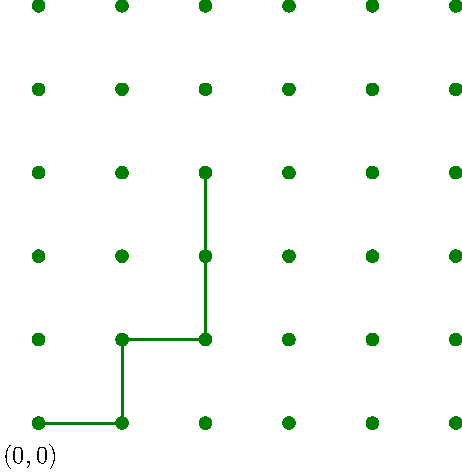
\includegraphics[width=5cm]{C2007_1.pdf}
  % C2007_1.pdf: 283x283 px, 72dpi, 9.98x9.98 cm, bb=0 0 283 283
  \caption{Chemins sur une grille}
  \label{fig:C2007_1}
\end{figure}

On considère une grille formée de points à coordonnées entières. Un chemin est constitué de segments: un point $M$ de coordonnées $(x,y)$ est l'origine de deux segments seulement
\[
 M-(x+1,y) \text{ segment horizontal }, \hspace{0.5cm} M-(x,y+1) \text{segment vertical}. 
\]
Pour un entier $n$ non nul, l'ensemble des chemins de longueur $n$ issus d'un point donné est en bijection avec l'ensemble des parties de $\llbracket 1,n\rrbracket$.
\begin{demo}
 Fixons arbitrairement l'origine des chemins à $(0,0)$. Soit $A$ une partie de $\llbracket 1,n \rrbracket$. On lui associe le chemin de longueur $n$ constitué des segments $(S_1,\cdots, S_n)$ tels que 
 \[
  S_i \text{ horizontal } \Leftrightarrow i \in A. 
 \]
Par exemple, pour $n=5$ et $A = \left\lbrace 1,3,4 \right\rbrace$, le chemin associé est
\[
 (0,0) \rightarrow (1,0)\rightarrow (1,1) \rightarrow (2,1) \rightarrow (2,2) \rightarrow (2,3).
\]
Voir figure \ref{fig:C2007_1}. La fonction ainsi définie est une bijection car tout chemin de longueur $n$ est caractérisé par la place de ses segments horizontaux.
\end{demo}
Soit $M_1 = (x_1,y_1)$ et $M_2 = (x_2,y_2)$ avec $x_1 \leq x_2$ et $y_1 \leq y_2$. Le nombre de chemins issus de $M_1$ et aboutissant à $M_2$ est 
\[
\binom{x_2 - x_1 + y_2 - y_1}{x_2 - x_1}. 
\]
\begin{demo}
 Tous les chemins de $M_1$ vers $M_2$ sont de longueurs $l = x_2 - x_1 + y_2 - y_1$ et constitués de $x_2 - x_1$ segments horizontaux et $y_2 - y_1$ segments verticaux. Un tel chemin est caractérisé par la place dans $\llbracket 1,n \rrbracket$ des $x_2-x_1$ segments horizontaux d'où la formule.
\end{demo}
\clearpage
\subsection{Formule du binôme}
On peut utiliser les images précédentes pour démontrer directement la formule du binôme. 
\begin{demo}
Considérons de éléments $h_1,\cdots, h_n$ et $v_1,\cdots,v_n$. Ils appartiennent à un anneau quelconque mais doivent commuter entre eux.\newline
Développer c'est choisir. Pour illustrer cela développons 
\[
 T = (h_1 + v_1)(h_2 + v_2) \cdots (h_n + v_n).
\]
On obtient une somme de $2^n$ termes et chaque terme est un produit de $n$ facteurs: certains sont des $h_i$ d'autres des $v_j$. Rassemblons les $h_i$ et les $v_i$
\[
 T = \sum_{A \in \mathcal{P}(\llbracket 1,n \rrbracket)} \left( \prod_{i\in A}h_i\right) \left( \prod_{i \notin A}v_i\right).
\]
Supposons tous les $h_i$ égaux à $h$ et tous les $v_j$ égaux à $v$. Rassemblons les parties avec le même nombre d'éléments:
\[
 (h + v)^n = T = \sum_{A \in \mathcal{P}(\llbracket 1,n \rrbracket)} h^{\sharp A}\, v^{n - \sharp A}
 = \sum_{k = 0}^{n}\sum_{A \in \mathcal{P}_k(\llbracket 1,n \rrbracket)} h^{k}\, v^{n - k}
 = \sum_{k = 0}^{n}\binom{n}{k} h^{k}\, v^{n - k}.
\] 
\end{demo}


\end{document}
